\documentclass[a4paper]{report}
\usepackage[utf8x]{inputenc}
\usepackage[T1]{fontenc}
\usepackage[french]{babel}
\usepackage{graphicx}
\usepackage{footmisc}
\usepackage{fullpage}
\usepackage{eso-pic}
\usepackage{hyperref}
\usepackage{textcomp}
\usepackage{float}
\usepackage{appendix}
\usepackage{amsthm}
\usepackage{amsmath}
\usepackage{listings}
\usepackage{color}
\usepackage{subcaption}



\usepackage{array}

\definecolor{codegreen}{rgb}{0,0.6,0}
\definecolor{codegray}{rgb}{0.5,0.5,0.5}
\definecolor{codepurple}{rgb}{0.58,0,0.82}
\definecolor{backcolour}{rgb}{0.95,0.95,0.92}

\lstdefinestyle{mystyle}{
    backgroundcolor=\color{backcolour},
    commentstyle=\color{codegreen},
    keywordstyle=\color{magenta},
    numberstyle=\tiny\color{codegray},
    stringstyle=\color{codepurple},
    basicstyle=\ttfamily\footnotesize,
    breakatwhitespace=false,
    breaklines=true,
    captionpos=b,
    keepspaces=true,
    numbers=left,
    numbersep=5pt,
    showspaces=false,
    showstringspaces=false,
    showtabs=false,
    tabsize=2
}



\lstset{style=mystyle}
%\renewcommand{\thesection}{\arabic{section}}

%%\renewcommand\lstlistingname{Quelltext} % Change language of section name

%\providecommand{\tightlist}{%
%temsep}{0pt}\setlength{\parskip}{0pt}}

\providecommand{\tightlist}{}

\newcommand{\HRule}{\rule{\linewidth}{0.5mm}}
\newcommand{\blap}[1]{\vbox to 0pt{#1\vss}}
\newcommand\AtUpperLeftCorner[3]{%
  \put(\LenToUnit{#1},\LenToUnit{\dimexpr\paperheight-#2}){\blap{#3}}%
}
\newcommand\AtUpperRightCorner[3]{%
  \put(\LenToUnit{\dimexpr\paperwidth-#1},\LenToUnit{\dimexpr\paperheight-#2}){\blap{\llap{#3}}}%
}

\title{\LARGE{\begin{center}MÉMOIRE DE STAGE\end{center} \leavevmode\newline Résolution de Sudoku}}
\author{\textsc{Minatchy} Jérôme\\M1 Informatique\\Année universitaire 2020/2021 à rendre pour le 3 Juin 2021}
\date{\today}
\makeatletter

\begin{document}
\begin{titlepage}
    \enlargethispage{2cm}

    \AddToShipoutPicture{
        \AtUpperLeftCorner{1cm}{0.5cm}{
\includegraphics[width=4cm]{./images/logoUA.jpg}}
    }
    \begin{center}
        \vspace*{1cm}
        
\includegraphics[width=6.5cm]{./images/lamialogo.jpg}
        \vspace*{0.5cm}

        \textsc{\@title}
        \HRule
        \vspace*{0.5cm}

        \large{\@author}
    \end{center}

    \begin{center}
      \vspace*{2cm}
      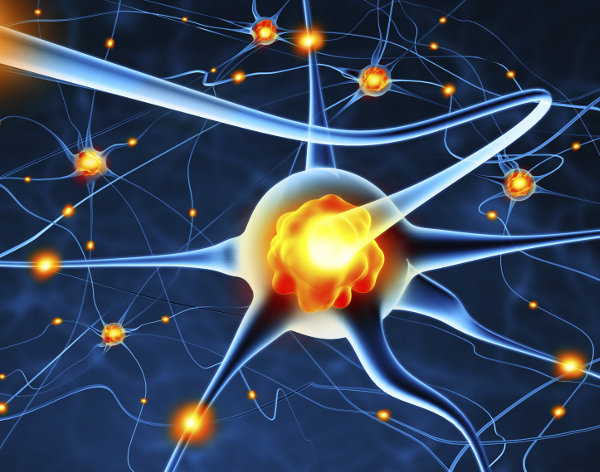
\includegraphics[width=6.5cm]{./images/n_a.jpg}
    \end{center}

    \vspace*{2cm}

    \begin{center}
        Université des Antilles

        (Entreprise d'accueil)
        %\makebox[\textwidth]{
\includegraphics[width=\paperwidth]{./images/logoUA.jpg}}
    \end{center}

\end{titlepage}
\ClearShipoutPicture

\listoffigures
\tableofcontents

\hypertarget{Introduction}{%
\chapter{Introduction}\label{Introduction}}

\section{Présentation de la structure
d'accueil}

Durant la période de mon stage , j'ai été accueilli au
\textbf{Laboratoire de Mathématiques Informatique et Application
(LAMIA)} de l'Université des Antilles (UA).

Pour présenter cette structure, il me faut tout d'abord présenter
l'université à laquelle il est rattaché.

\hypertarget{luniversite-des-antilles}{%
\subsection{L'université des Antilles}\label{luniversite-des-antilles}}

Bien que ce soit l'université dans laquelle j'ai fait toutes mes études,
voici quelques chiffres que je ne connaissais pas et qui donnent la
mesure de sa taille :

L'Université des Antilles s'organise autour deux pôles universitaires
régionaux autonomes : le « Pôle Guadeloupe » et le « Pôle Martinique ».

Sur ces pôles, l'Université assure des missions d'\emph{enseignement} et
de \emph{recherche}, assistées par des \emph{administratifs et des
techniciens}.

\hypertarget{administration-et-personnel-technique}{%
\subsubsection{Administration et personnel
technique}
\label{administration-et-personnel-technique}}

l'UA emploie 414 Administratifs et Techniciens (environ 200 personnes
pour l'administation centrale et 100 répartis sur chaque pôle)

\hypertarget{enseignements}{%
\subsubsection{Enseignements}\label{enseignements}}

L'UA délivre des diplomes de la licence au doctorat dans de nombreux
domaines. Au total, cela représente :

\begin{itemize}
\tightlist
\item
  484 enseignants-chercheurs (environ 240 pour chaque pôle)
\item
  12 000 étudiants (environ 7000 pour la Guadeloupe , 5000 pour la
  Martinique)
\end{itemize}

Pour l'informatique, cela représente : - autour de 20
enseignants-chercheurs - autour de 120 étudiants

\hypertarget{le-lamia}{%
\subsection{Le LAMIA}\label{le-lamia}}

Le \textbf{Laboratoire de Mathématiques Informatique et Application
(LAMIA)}, comme son nom l'indique, se concentre sur les recherches en
informatiques et mathématiques.

Il compte une soixantaine de membres (Professeurs des Universités,
Maitres de Conférences, ATER, Doctorants) répartis sur deux pôles
(Guadeloupe et Martinique) au sein de trois équipes internes :

\begin{itemize}
\tightlist
\item
  Equipe
  \href{http://lamia.univ-ag.fr/index.php?page=equipe-mathematiques}{\textbf{Mathématiques}
  (analyse variationnelle, analyse numérique, EDP, analyse statistique,
  mathématiques discrètes)} ;
\item
  Equipe Informatique
  \href{http://lamia.univ-ag.fr/index.php?page=equipe-danais}{\textbf{DANAIS}
  : Data analytics and big data gathering with sensors} ;
\item
  Equipe Informatique
  \href{http://lamia.univ-ag.fr/index.php?page=equipe-aid}{\textbf{AID}
  : Apprentissages Interactions Donnees} ;
\end{itemize}

De plus, le LAMIA accueille en son sein un groupe de chercheurs associés
travaillant en Epidémiologie clinique et médecine.



\hypertarget{contexte-guxe9nuxe9ral}{%
\section{Contexte général}\label{contexte-guxe9nuxe9ral}}


\hypertarget{Etat de l'art}{%
\section{Etat de l'art}\label{Etat de l'art}


\hypertarget{Méthodologie}{
\section{Méthodologie}\label{Méthodologie}}
\subsection{Outils utilisés}



\subsubsection{Présentation de Python}

\begin{figure}[h]
  \begin{center}
  
\includegraphics[width=4cm]{./images/Python_Logo.png}\label{Python}
  \caption{Logo de Python.}
  \end{center}
\end{figure}

Python est un langage de programmation interprété\footnote{\label{interprete}Langage nécéssitant un programme informatique qui joue le rôle d’interface entre le projet et le processeur appellé interpréteur, pour exécuter du code.} qui sera utiliser pour l'ensemble du projet. Nous avons choisi ce langage car il n'y a pas beaucoup de résolution

\subsubsection{Présentation Qt}

\begin{figure}[h]
  \begin{center}
  
\includegraphics[width=2cm]{./images/Qt_logo_2016.png}\label{Qt}
  \caption{Logo de Qt.}
  \end{center}
\end{figure}

QT est une librairie\footnote{\label{librairie}Une librairie est un fichier contenant du code (généralement un ensemble de fonction et classes permettant de faciliter et/où de réaliser certain programme)} qui permet le création d'interface graphique en Python.Que nous utiliserons pour créer l'interface que l'on utilisera au cours du projet.

\subsubsection{Présentation Cplex}

\begin{figure}[h]
  \begin{center}
  
\includegraphics[width=4cm]{./images/cplex.png}\label{Cplex}
  \caption{Logo de Cplex.}
  \end{center}
\end{figure}

Cplex est une librairie\footref{librairie} qui permet la modélisation et la résolution de problème d'optimisation linéaire\footnote{Terme que j'expliquerais plus tard dans mon rapport}.
\newline
\newline
\subsubsection{Présentation de GitHub}
\begin{figure}[h]
  \begin{center}
  
\includegraphics[width=3cm]{./images/github.jpg}\label{GitHub}
  \caption{Logo de GitHub.}
  \end{center}
\end{figure}


Nous pouvons définir GitHub comme une plateforme de développement de projet informatique en groupe. Elle simplifie grandement le développement de projets. Elle permet de versioner ses programmes et d'y apporter des modifications en temps réel à plusieurs.

\subsubsection{Présentation de LaTex}

\begin{figure}[h]
  \begin{center}

\includegraphics[width=2cm]{./images/Latex.png}\label{LaTex}
\caption{Logo de LaTex}
\end{center}
\end{figure}

Nous pouvons dire que LaTex est un langage de traitement de texte tel que le markdown qui permet de mettre en forme notre texte de manière \"scientifique\" cela veut dire que. LaTex permet une faciliter d'écriture des équations et de toutes les écriture mathématiques.Permet de par ses nombreux package une quasi-infinité de possibilitées.
L'utilisation de cet outil permettra une synergie entre ceux-ci car LaTex peut-être utiliser avec un simple bloc-note c'est donc du texte ce qui permet une intéraction facilitée avec GitHub d'ailleurs ce rapport est écrit avec Latex et retrouvable sur GitHub.\newline


\hypertarget{Annonce du plan}{%
\section{Annonce du plan}\label{annonce du plan}}

\subsection{Présentation des stratégies de résolution}

Dans cette première partie je commencerais par vous présenter la première solution de résolution choisie qui est la résolution du sudoku en tant que problème d'optimisation linéaire.\newline
Je vous expliquerai ce qu'est un problème d'optimisation linéaire puis vous décrirai l'algorithme du simplex qui nous permettra de le résoudre.\newline
En deuxième grande sous partie de cette section je vous présenterai l'algorithme du backtraking.\newline
En dernière sous partie de cette présentation je vous expliquerai pourquoi le choix de ces deux solutions.
\subsection{Implémentation des stratégies}
La première sous partie de cette grande sous partie commencera avec la modélisation et l'implémentation d'un sudoku en python et l'implémentation de l'interface graphique.\newline
La seconde sera l'implémentation de la méthode résolution utilisant cplex.\newline
Pour finir nous ferons l'implémentationde la méthode utilisant l'algorithme du backtracking.\newline
\subsection{Test du résolveur}
Nous commencerons par établir nos méthodes de test, expliquer la raison du choix de ces test.\newline
Nous continuerons avec l'implémentation de ceux-ci.\newline
Nous finirons par présenter et analyser nos résultats.\newline
\subsection{Conclusion}
Nous terminerons ce rapport par une conclusion où nous rappelerons brièvement la problématique.\newline
Nous ferons le bilan des produits du projet de stage.\newline
Nous ferons le bilan des apports du stage.\newline
Et finirons par une ouverture en étudiants nos perspectives.

\hypertarget{Déroulement}{%
\chapter{Déroulement}\label{Déroulement}}

Ce chapitre, le plus volumineux du rapport, décrira l'ensemble des tâches que j'ai eu à effectuer au cours de ces deux mois.


\section{Présentation des stratégies de résolution}
\subsection{Présentation de la résolution avec Cplex}
\subsubsection{Qu'est-ce qu'un problème d'optimisation linéaire}
Nous allons dans cette première partie parler de la résolution de sudoku comme étant un problème d'optimisation linéaire. Mais tout d'abord nous devons définir ce qu'est un problème d'optimisation linéaire.\newline\newline
Par définition un problème d'optimisation linéaire est un problème dont la valeur à obtimiser ainsi que les contraintes qui y seront appliquer peuvent-êtres modélisées sous la forme d'une fonction linéaire cette description n'est pas des plus précises que l'on puisse c'est pour cela que nous allons l'étoffer par un problème connu.\newline\newline
Le problème du brasseur de bière peut être énoncer comme suit:\newline\newline
Un brasseur fabrique 2 types de bières : blonde et brune.\newline
3 ingrédients : maïs , houblon , malt.\newline
Quantités requises par unité de volume:\newline
Bière blonde: 2,5 kg de maïs, 125 g de houblon, 17,5 kg de malt\newline
Bière brune : 7,5 kg de maïs, 125 g de houblon, 10 kg de malt\newline
Le brasseur dispose de 240 kg maïs, 5 kg houblon , 595 kg malt\newline
Prix vente par u.v. : blonde 9 euros , brune 15 euros
Le brasseur veut maximiser son revenu .\newline
Quelle quantité de bières blondes et/ou brunes doit-il produire pour cela ?\newline
\newline
Nous pouvons modéliser le revenu du brasseur comme étant une fonction linéaire tel que:\newline
Soit $x^{1}$ le nombre de volumes d'unité de bière blonde et $x^{2}$ le nombre d'unité de volume de bière brune\newline
Nous avons:\newline\newline
Le revenu que nous de vons maximiser: $R = x^{1}*9 + x^{2}*15$\newline\newline
Les contraintes peuvent êtres représentées comme suit:\newline\newline
La quantité maximale de maïs: $M \geq x^{1}*2,5+x^{2}*7,5$\newline
La quantité maximale de houblon: $H \geq x^{1}*0,125+x^{2}*0,125$\newline
La quantité maximale de malt: $Ma \geq x^{1}*17,5+x^{2}*10$\newline\newline

\subsubsection{Comment résoudre un problème d'optimisation linéaire}

 Maintenant que nous avons vu ce qu'est un problème d'optimisation linéaire et illustré ceci par un exemple nous allons voir comment peut-on le résoudre plus particulièrement comment avec l'algorithme du simplex en théorie puis avec Cplex.

 La résolution avec cplex est des plus simples il suffit de mettre en place nos contraintes et notre fonction à maximiser le code sera donner et expliciter en annexe:

 \begin{figure}[h]
   \begin{center}
 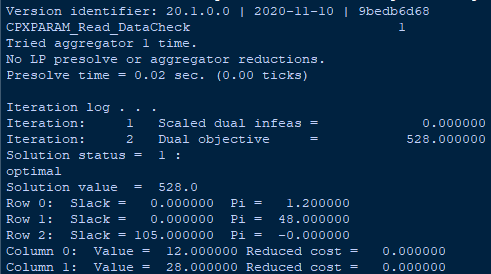
\includegraphics[width=10cm]{./images/Brasseur_Resolution.png}\label{Resultat_Brasseur}
 \caption{Résultat de l'optimisation du problème du brasseur}
 \end{center}
 \end{figure}

Nous voyons que nous avons pour revenu maximum 528 euro avec 12 unité de volume de bière blonde produite et 28 uinité de bière brune produites.

\subsection{Présentation de la résolution par backtracking}
L'algorithme du backtracking est plus précisément une famille d'algorithme qui sont utilisé le plus souent pour résoudre des problmèmes de satisfaction de contrainte.
Le backtracking est la solution la plus simple à comprendre il s'agit tout simplement de tester toutes les valeurs possible sur chaque case jusqu'a obtenir une sortie de sudoku remplie et valide.Cette algorithme agit comme un parcours d'arbre illustrons cela avec une image:\newline

\begin{figure}[h]
  \begin{center}
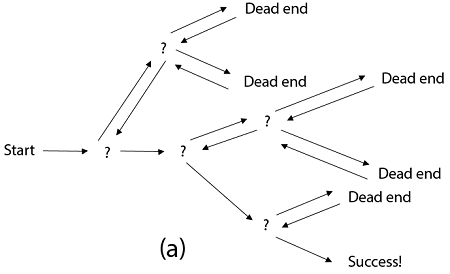
\includegraphics[width=10cm]{./images/backtracking.png}\label{Backtracking}
\caption{Illustration de l'algorithme du backtracking.}
\end{center}
\end{figure}

Comme l'illustre cette image nous essayons toutes les possibilitées et retournons en arrière si nous tombons dans une impasse dans nous passons de case vide\footnote{\label{vide}Une case vide est comme dit plus haut une case contenant la valeur 0} en case vide\footref{vide} en revenant en arrière si peu importe la le chiffre essayer dans cette case allant de 1 à 9, nous donne un sudoku invalide. Le problèlme de cette algorithme qui reviens le plus souvent est dù au fait que nous essayons toutes les valeurs possible ce qui nous donne une très grande quantité d'action et donc ce qui augmente considérablement notre temps de calcul nous pouvons toutefois régler ce problème en évitant de tester les possibiliter qui nous amène de façon logique à une impasse ou éviter de tester des possibilité d'une case si il est possible de déduire sa valeur de façon logique.
\subsection{Pourquoi utiliser ces deux algorithme}

\subsubsection{Pourquoi utiliser l'algorithme du simplex}

La résolution avec l'algorithme du simplex permet une implementation intuitive et facililité dù à l'utilisation de Cplex. Cplex nous permet aussi une meilleur étude de la complexité de notre algorithme car cous pouvons voir les différentes itération de recherche de notre outil de résolution. Cette méthode de résolution nous permet aussi de revoir le problème de plusieur façon différente de par le fais que la résolution ne dépends que de nos contraintes.

\subsubsection{Pourquoi utiliser l'algorithme utilisant le backtracking}

La résolution avec avec backtracking est l'algorithme le plus naturel qui viennent à l'esprit dans la résolution de problème avec contrainte ce qui permet une facile implémentation de la gestion des contraintes malgré leur nombre.C'est un algorithme facilement améliorable car le but tout au long de son implémentation sera de tester le moins de valeur menant à une impasse possible. Cette algorithme a aussi pour avantage de n'avoir besoin daucune librairie extérieur ce qui permet une liberté totale au niveau du code et donne lieu à une certaine transparence quand à son fonctionnement contrairement aux au code que nous utilisons via cplex qui peuvent différé légèrement de leurs fonctionnements théoriques cités plus haut.

\subsection{Implémentation des Stratégies de résolution}

\subsection{Modélisation et implémentation d'un sudoku en Python et de l'interface graphique}


Nous allons stocker dans une liste\footnote{\label{liste_Python}structure de donnée incluse de base dans python qui permet de contenir plusieurs variables différentes} contenant 9 listes\footref{liste_Python} qui représenteront nos ligne qui elles contiendront 9 entiers allant de 0 à 9. Nous aurons donc besoin de coder des fonctions pour faire le lien entre l'interface et notre résolveur du fait de notre modélisation du sudoku nous pouvons découper cela en plusieurs fonction utilitaire:\newline
\begin{itemize}
\item Une fonction qui nous permettra de stocker le contenu de notre interface graphique dans une liste comme celle décrite précédemment
\item Une fonction permettant de transférer le contenu d'une liste comme celle décrite plus haut dans notre interface graphique
\item Une fonction permettant de copier le contenu de la zone de saisi de notre interface dans la zone d'affichage de notre interface
\item Une fonction permettant de copier le contenu de la zone d'affichage de notre interface dans la zone de saisi de notre interface
\end{itemize}

\hypertarget{conclusion}{%
\chapter{Conclusion}\label{conclusion}}

\section{Rappel de la problèmatique}

Notre problèmatique à la base était la résolution de sudoku Standart ce que nous avons reussi. Nous avons donc pour avoir une autre vision du problème nous avons choisi de généraliser celui-ci. Ce qui nous a ouvert à des pistes d'améliorations dont nous n'aurions pas eu besoin dans le cas de la résolution de sudoku.

\section{Réponse apportées}

\section{Piste d'amélioration}
Nous pourrions pour voir les limite de l'algorithme du Cplex l'utiliser sur un grand volume de sudopku et voir le temps mis pour tous les résoudre en une seule fois. Nous pourrions essayer avec des sudokus d'une taille extrème pour en vérifier la consistence.\newline Comme dit précédemment en ce qui concerne la déduction des valeur nous pouvons évviter beaucoup de test inutiles grace à cela.

\section{Les apports du stage}

\subsection{les apports a l'entreprise}

\subsection{les apports personels}


\section{Perspectives}

\chapter{Remerciements}\label{Remerciements}
Je souhaiterais addresseé mes remerciements:
\begin{itemize}
  \item Monsieur Andrei Doncescu qui m'a proposé ce stage et qui a été mon maître de stage durant tout ce projet.
  \item Le LAMIA d'avoir pu m'accueillir en son sein.
  \item Mon collègue stagiaire stéphane qui m'a aidé dans la recherche de document
\end{itemize}


\cleardoublepage
\phantomsection
\bibliographystyle{plain} % Le style est mis entre accolades.
\addcontentsline{toc}{chapter}{Bibliographie}
\bibliography{biblioMinatchy}


\appendix

\chapter{Annexes}

%\include{bases}

\end{document}
